\documentclass[tikz]{standalone}
\usepackage{framed}
\usepackage{amsmath} 
\usepackage{amsfonts}
\DeclareMathOperator{\f}{f}
\usepackage{xcolor}

\usetikzlibrary{shadows.blur}
\usetikzlibrary{arrows}
\usetikzlibrary{positioning}

\begin{document}
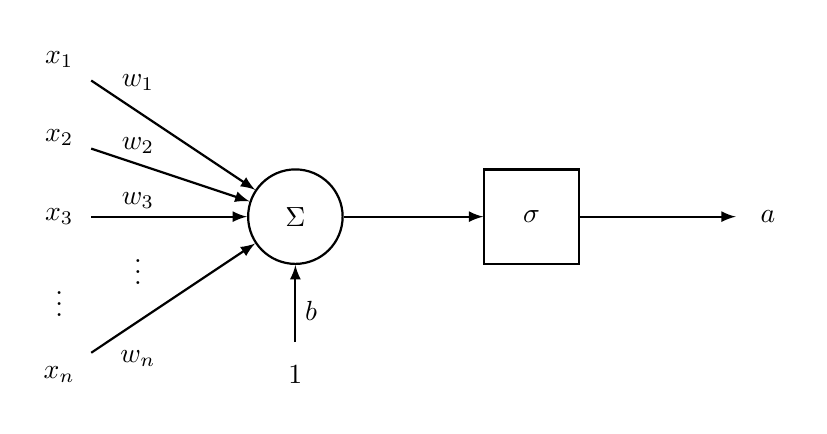
\begin{tikzpicture}[]
	%\draw[help lines] (-2,0) grid (20,10);
	
	\tikzstyle{inode} = [minimum size=8mm]
	\tikzstyle{vnode} = [circle,draw,thick,fill=white,minimum size=12mm]
	\tikzstyle{snode} = [rectangle,draw,thick,fill=white,minimum size=12mm]
	\tikzstyle{vedge} = [->,>=latex,thick]
	
	
	\node[inode] (x1) at (-9, 2) {$x_1$};
	\node[inode] (x2) at (-9, 1) {$x_2$};
	\node[inode] (x3) at (-9, 0) {$x_3$};
	\node[inode] (xdots) at (-9, -1) {$\vdots$};
	\node[inode] (xn) at (-9, -2) {$x_n$};
	\node[inode] (xb) at (-6, -2) {$1$};
	
	\node[inode] (w1) at (-8, 1.7) {$w_1$};
	\node[inode] (w2) at (-8, 0.9) {$w_2$};
	\node[inode] (w3) at (-8, 0.2) {$w_3$};
	\node[inode] (wdots) at (-8, -0.6) {$\vdots$};
	\node[inode] (wn) at (-8, -1.8) {$w_n$};
	\node[inode] (wb) at (-5.8, -1.2) {$b$};

	\node[vnode] (n) at (-6, 0) {$\Sigma$};

	\node[snode] (f) at (-3, 0) {$\sigma$};
	
	\node[inode] (o) at (0, 0) {$a$};
	
	\draw (x1) edge [vedge] (n);
	\draw (x2) edge [vedge] (n);
	\draw (x3) edge [vedge] (n);
	\draw (xn) edge [vedge] (n);
	\draw (xb) edge [vedge] (n);
	\draw (n) edge [vedge] (f);
	\draw (f) edge [vedge] (o);

\end{tikzpicture}
\end{document}
